\documentclass{report_template_oxford}

\title{3YP Report}
\subtitle{Multiagent Autonomous Drone System for Landmine Detection}
\author{Group B: Huirui Dai, Samuel Grace, Rory Millard, Jihwan Shin, Thomas Turner}
\date{March 2025}

\begin{document}
\maketitle

% Abstract
% - Concise summary of report
% - Naming of essential outcomes
% - As short as possible while providing key points
% - Less than 1 page
\pagenumbering{roman}
\newpage
\addcontentsline{toc}{section}{Abstract}
\fancyhead[C]{Student author of section}
\section*{Abstract}

Add abstract here.

\newpage
\fancyhead[C]{}
\tableofcontents

\newpage
\addcontentsline{toc}{section}{List of Figures}
\listoffigures

\newpage
\addcontentsline{toc}{section}{List of Tables}
\listoftables

\newpage
\addcontentsline{toc}{section}{Glossary}
\printglossaries

\newpage
\pagenumbering{arabic}
\fancyhead[C]{Student}
\section{Introduction} \label{introduction}

\fancyhead[C]{Student}
\subsection{Sub-Introduction}

%\newpage
\pagenumbering{arabic}
\fancyhead[C]{Jihwan Shin}
\section{Mission Planning} \label{missionplanning}

In \gls{cpp} we must cover the entire region of interest \cite{cabreira2019cpp}. As mentioned in section~\ref{hardware}, we will use thermal and GPSAR sensors.

%\newpage
\pagenumbering{arabic}
\fancyhead[C]{Huirui Dai}
\section{Hardware} \label{hardware}

%\newpage
\pagenumbering{arabic}
\fancyhead[C]{Rory Millard}
\section{Computer Vision} \label{computervision}

\subsection{Thermal Computer Vision}

This is the thermal computer vision subsection
\subsection{Thermal Simulations}

This is the thermal simulations subsection

\subsubsection{Governing Equations}
Unsteady Heat Equation

The general form of the 3D unsteady heat equation in Cartesian coordinates is:

\begin{equation}
    c_p \rho \frac{\partial T}{\partial t} = 
    \frac{\partial}{\partial x} \left( k \frac{\partial T}{\partial x} \right) + 
    \frac{\partial}{\partial y} \left( k \frac{\partial T}{\partial y} \right) + 
    \frac{\partial}{\partial z} \left( k \frac{\partial T}{\partial z} \right)
\end{equation}


where:
\begin{itemize}
    \item \( T(x,y,z,t) \) is the temperature field,
    \item \( k(x,y,z,t) \) is the thermal conductivity,
    \item \( \rho(x,y,z,t) \) is the mass density,
    \item \( c_p (x,y,z,t) \) is the specific heat capacity.
    
\end{itemize}

For piecewise constant properties $\rho, k, c_p$ this can be written as

\begin{equation}
    \frac{\partial T}{\partial t} = \alpha \left( \frac{\partial^2 T}{\partial x^2} + \frac{\partial^2 T}{\partial y^2} + \frac{\partial^2 T}{\partial z^2} \right)
\end{equation}

which can be compactly written as

\begin{equation}
    \frac{\partial T}{\partial t} = \alpha \nabla^2 T
\end{equation}



Where \( \alpha(x,y,z,t) := \frac{k}{\rho c_p}\) is the thermal diffusivity.


\subsection{Radar Computer Vision}

This is the radar computer vision subsection
\subsection{Radar Simulations}

This is the radar simulations subsection

\subsection{Data Fusion}

This is the data fusion subsection

%\newpage
\fancyhead[C]{Rory Millard}
\section{Sensor Fusion} \label{fusion}



\subsection{Overview of Fusion} \label{fusion_overview}

    \noindent The late stage fusion approach was introduced in Section \ref{compvis_intro}. It is justified on the grounds of simplicity; by processing each sensor's data through individual YOLO models before merging, the network architectures are simpler. The networks can be retrained in parallel, and single points of failure are removed. 
    


    \noindent In this section, the outputs from the individual YOLO models are interpreted as probability maps, where the confidence value assigned by the YOLO model is equal to the probability of finding a landmine at that location, according to each sensor. The fusion algorithm combines the two probability maps, defined over the same geographical space, into a third map. This is done using the sensor data and environmental contextual data.

    Fusing the sensor outputs before the CNN is problematic due to irregular input sizes and the need for computationally intensive mosaicking algorithms that may introduce errors. Instead, the accurate position, pose and field of view metadata  is leveraged to project each YOLO output onto a common geographical grid. Given that these probability maps are inherently sparse (most of the probability map is zero, with occasional spikes over landmines), the projections are computationally efficient. Because the metadata is accurate, the overlapping regions of the projections will be small, and when they occur, a simple strategy—such as weighted averaging—suffices to resolve them.

    \subsubsection{The Precision-Recall Trade-off } \label{lossmatrix}

        Recall should be prioritized over precision, as a false negative in landmine detection is more dangerous than a false positive. However, no system can ensure 100\% recall, and so a mined region can never be 100\% safe. Therefore, reducing recall slightly in exchange  for a significant gain in precision can be advantageous, because the reduced recall has negligible operational impact, whilst the increased precision is associated with significant cost reduction.
\subsection{Fusion System Performance Bounds}\label{fusion_bounds}

    Independent of the specific fusion algorithm employed, the overall system performance is ultimately constrained by the intrinsic capabilities of the individual sensors. A Naive Bayes framework is adopted to establish performance estimates. The Naive Bayes approach assumes conditional independence between sensors, allowing for straightforward analytical expressions of posterior probabilities. While this simplification may not perfectly capture all sensor interactions, it provides tractable mathematics that yield conservative performance estimates; algorithms that are not limited by conditional independence, and have access to domain knowledge, will perform better than Naive Bayes for fusion.

    \subsubsection{Theoretical Framework}
        
        The following key parameters and their probabilistic interpretation, are defined: the prior mine density $\rho_0 = P(\text{Mine})$, the set of locations that have been flagged by the thermal sensor \(\mathcal{T}^+\), the thermal sensor's recall $R_T = P(\mathcal{T}^+\mid\text{Mine})$ , and its false positive rate $F_T = P(\mathcal{T}^+ \mid \overline{\text{Mine}})$. Similarly, the radar sensor is characterized by its recall $R_R$ and false positive rate $F_R$ with analagous interpretations. Following thermal scanning, the mine density in the flagged region ($\rho_1$), can be found with Bayes rule:
        \begin{equation}
        \rho_1 = P(\text{Mine} \mid \mathcal{T}^+) =\frac{P(\mathcal{T}^+\mid\text{Mine})P(\text{Mine})}{P(\mathcal{T}^+\mid\text{Mine})P(\text{Mine})+ P(\mathcal{T}^+\mid \overline{\text{Mine}})P(\overline{\text{Mine}})} =\frac{R_T \rho_0}{R_T \rho_0 + F_T (1 - \rho_0)}
        \end{equation}
        
        \paragraph{Mine Densities} 
        

            Note the use of mine densities (\(\rho\)) rather than the nominal precision values reported in Section \ref{compvis_implementation}. This is because of the class imbalance discussed in Section \ref{class_imbalance}. The nominal precision derived from an imbalanced dataset is misleading when applied to real-world conditions. Instead, a full Bayesian treatment that incorporates the prior distribution over mine density is used. This enables the accurate updating of mine density after thermal screening, giving \(\rho_1\), and then after radar verification, giving \(\rho_2\), thereby mitigating the effects of class imbalance.

    \subsubsection{Bounds on Precision and Recall}
    
        \paragraph{Precision} Under the Naive Bayes framework, the expected system precision after fusion equals the posterior mine density after both sensors have flagged an area. The radar sensor refines the density from $\rho_1$ to $\rho_2$, and the expected precision after fusion is:
        \begin{equation}
        \label{eq:rho_2}
        P_\text{F} = \rho_\text{2} = \frac{R_\text{R} \rho_\text{1}}{R_\text{R} \rho_\text{1} + F_\text{R} (1-\rho_\text{1})} \text{, where }         \rho_\text{1} = \frac{R_\text{T} \rho_\text{0}}{R_\text{T} \rho_\text{0} + F_\text{T} (1-\rho_\text{0})}.
        \end{equation}
        
         The upper bound is the radar's intrinsic precision $P_\text{R}$, giving \textbf{precision bounds of } $\rho_\text{2} \leq P_\text{sys} < P_\text{R}$
         
        \paragraph{Recall} The Naive Bayes system recall can similarly be found by considering the intrinsic recalls of each sensor, and is a lower bound on the true system recall. Because the radar sensor only scans regions flagged by the thermal sensor, the NB system recall is the product of the individual recalls \(R_\text{sys} = R_\text{T} R_\text{R}\), 
        which  cannot exceed $R_\text{T}$. This gives the \textbf{bounds on the fused system's recall as} $R_\text{T}R_\text{R}\leq R_\text{sys}< R_\text{T}$.
    
    \subsubsection{Naive Bayes Fusion: Quantifying Bounds} \label{Rory_quantifying_bounds}
    
        Using the YOLO model performance metrics in Table \ref{tab:sensor_comparison}, and a prior landmine density of 2\% ($\rho_0 = 0.02$), the following values are obtained: $R_T = 0.919,~ F_T = 0.15,~ R_R = 0.833,~ F_R = 0.085.$ These values are used to calculate the posterior density after thermal screening and subsequent radar scanning, using Equation \ref{eq:rho_2}:
        \[
        P_{sys} \geq \rho_2 = \frac{R_R \rho_1}{R_R \rho_1 + F_R (1-\rho_1)} = \frac{0.833 \times 0.112}{0.833 \times 0.112 + 0.085 \times 0.888} \approx 0.553.
        \]
        
        Therefore, this fusion process concentrates the mine likelihood from an initial 2\% to \textit{at least} 55.3\% in the regions flagged by the radar sensor—\textbf{a  27.7× improvement over indiscriminate "blind" demining}. The expected system recall is $R_{sys} \geq R_T \times R_R \approx 0.919 \times 0.833 \approx 0.765$, indicating a maximum recall drop of about $0.919 - 0.765 \approx 15.3\%$ compared to using just the thermal sensor alone.


    \subsubsection{Implications for System Design}

        \paragraph{Benefit of the GPR Sensor}
        
            
            When the radar sensor is included as part of the layered architecture, the system precision is increased approximately 5 times, with only a marginal 15.3\% drop in recall. This trade-off is justified, as a modest reduction in recall has negligible operational impact (discussed in Section \ref{fusion_overview}), whilst the boost in precision dramatically reduces operational costs, which is mentioned in Section \ref{financing}. Therefore it is crucial to have the radar sensor.
                
        \paragraph{Benefit of the Layered Approach} \label{Benefit of the Layered Approach}
        
            The layered approach, where the radar sensor only probes the points flagged by the thermal sensor, enables the radar sensor to operate over a much smaller region, covering only $\rho_1 \approx 11.2\%$ of the total land area. In contrast, if both sensors were applied in parallel, with the radar sensor scanning the entire area, the detection time and hence cost would increase much (the radar sensor is significantly slower - Section \ref{sec:msp_comparison_manual_demining}), for only a slight improvement in recall and a negligible gain in precision. Therefore, the layered approach is a very efficient way of incorporating the radar sensor. 

            

        
\subsection{Explicit Fusion Algorithm Selection}

        An explicit fusion algorithm is required to intelligently combine the thermal and radar probability maps, \(\mathcal{P}_\text{thermal}(x, y)\) and \(\mathcal{P}_\text{radar}(x, y)\), respectively, into a final probability map, \(\mathcal{P}_\text{fused}(x, y)\), over the geographical area of interest. The selection of the fusion algorithm determines where the performance of the overall system lies within the bounds from Section \ref{fusion_bounds}, and requires careful consideration of the underlying assumptions and limitations of each method.
    
    \paragraph{Naive Bayes}
    
        An initial approach might be to use a Naive Bayes fusion algorithm. This approach was used as a conservative estimate on performance in Section \ref{fusion_bounds}, and assumes conditional independence between the sensor probability maps given the presence or absence of a landmine. 
        
        However, this assumption is fundamentally flawed in this context. The thermal and radar sensor readings are not independent; they are intrinsically linked by underlying causal physics. Factors such as soil moisture, ambient temperature, and vegetation cover influence both thermal signatures and radar reflections in complex, deterministic ways. A Naive Bayes model is incapable of capturing these dependencies, leading to inaccurate fusion results. This is validated in Section \ref{compvis_anfisvalid}.
    
    \paragraph{Kalman Filter}
    
        Similarly, the Kalman Filter, while offering a mathematically elegant framework for optimal linear estimation with Gaussian noise \footnote{\url{https://en.wikipedia.org/wiki/Kalman_filter}}, is ultimately unsuitable for this application. The Kalman Filter can model the sensor covariance \textit{statistically} but cannot encode causal, physical rules like \textbf{"low soil moisture fraction amplifies the thermal detectability"} (Section \ref{thermal_sensitivity}). This limits robustness in novel environments. More fundamentally though, the Kalman Filter's assumption of \textit{unbounded} Gaussian noise is violated in this case, where the variables are \textit{bounded} sensor confidence values, \(\mathcal{P}_{\text{thermal}}, \mathcal{P}_{\text{radar}} \in [0,1]\). Truncation of the output would introduce bias.
    
    \paragraph{Neural Network}

        A Neural Network (NN), as a universal function approximator, can learn arbitrarily complex mappings between sensor inputs and fused outputs. However, a standard NN cannot include domain knowledge without extensive training data. Even with ample data, a standard NN models the statistical behaviour of the physics, rather than the underlying causal mechanisms. This lack of domain understanding would cause poor performance in novel environments, for example: when the soil is frozen, there is no thermal contrast, so the thermal sensor data provides no useful information for buried landmine detection (this is used as a fuzzy rule in Section \ref{fuzzy_rules}).


    \paragraph{ANFIS}

        The Adaptive Neuro-Fuzzy Inference System (ANFIS) \cite{jang1993anfis} addresses the limitations of prior methods by hybridizing neural networks and physics-grounded fuzzy logic. Unlike Naive Bayes, ANFIS explicitly models dependencies between sensors through rules representative of causal physical relationships. By constraining solutions to physically plausible outcomes—such as suppressing thermal confidence in frozen soils—ANFIS can achieve robust fusion even in novel environments. The network effectively \textbf{learns the optimal rule weights} from data, ensuring that the fused predictions arise from first principles physics, rather than purely from statistical mimicry.


         \begin{figure}[htbp]
          \centering
          \begin{subfigure}[t]{0.48\textwidth} % Top-aligned subfigures
            \centering
            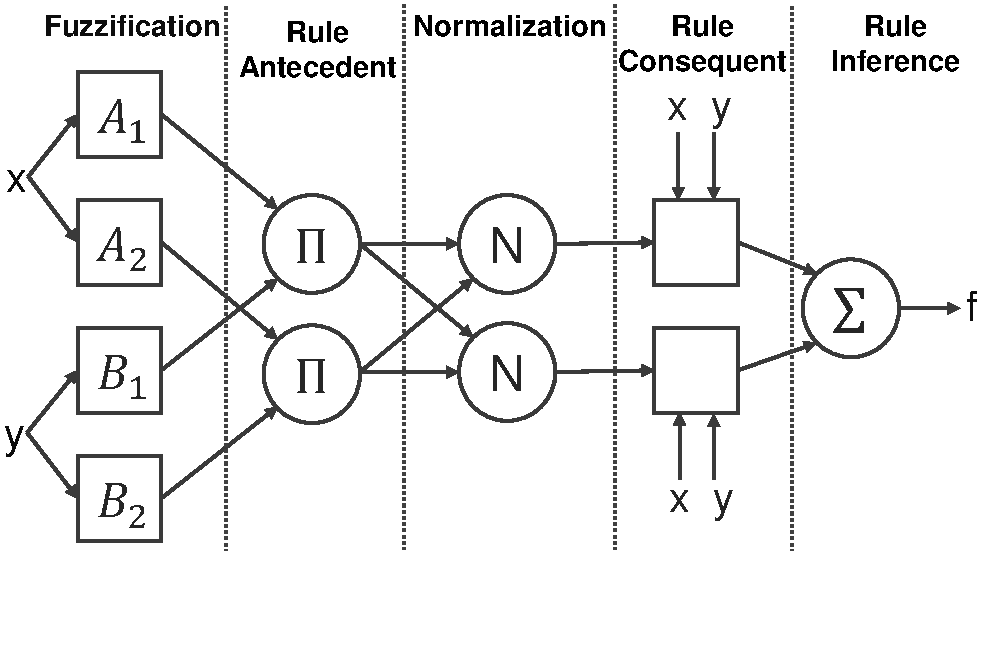
\includegraphics[width=\textwidth]{figs/Rory/ANFIS_diagram.pdf}
            \caption{}
            \label{fig:ANFIS_diagram}
          \end{subfigure}
          \hfill
          \begin{subfigure}[t]{0.48\textwidth} % Top-aligned subfigures
            \centering
            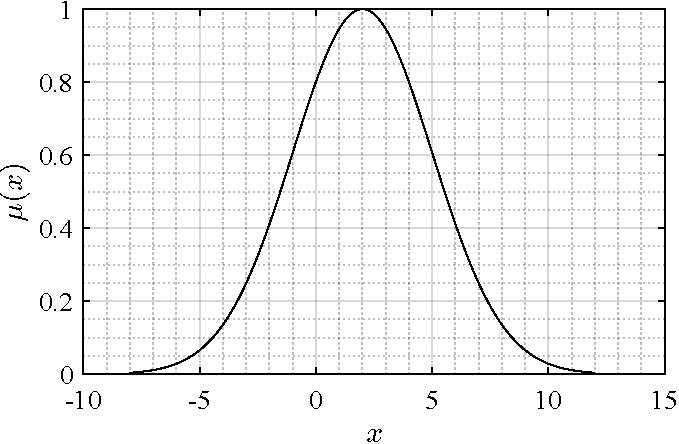
\includegraphics[width=\textwidth]{figs/Rory/mfs_plot.pdf}
            \caption{}
            \label{fig:membership_function_plot}
          \end{subfigure}
          \caption[ANFIS Network]{\textbf{a)} ANFIS network, with labelled layers. \textbf{b)} Gaussian membership function, with $c=2$ and $\sigma^2=9$.}
        \end{figure}

    
\subsection{ANFIS: Physics-Guided Fusion}

    \paragraph{Membership Functions}

        A fuzzy set is a linguistic representation of a numerical variable that has been fuzzified, enabling the modelling of uncertainty and partial truth. For example, the numerical range 1-10 can be categorised into the distinct fuzzy sets \textit{high, medium, low}. The value 9 would have a high \textit{degree of membership} in the fuzzy set \textit{high}, and a low degree of membership in the other sets. Membership functions are mathematical functions that assign each input value to a degree of membership \(\in [0,1]\) for each fuzzy set. 
        
        Gaussian membership functions have been chosen to represent the all of the environmental variables, and the sensor confidence values. The Gaussian membership function is defined as
        
        \[
        \mu(x) = \exp\left( -\frac{(x - c)^2}{2\sigma^2} \right),
        \]
        
        where \( c \) is the mode of the fuzzy set and \( \sigma^2 \) its variance, and is visualised in Figure \ref{fig:membership_function_plot}. This function is a smooth, differentiable bell curve.
        Gaussian membership functions are particularly well-suited for representing the natural variability in environmental parameters, such as soil moisture and ambient temperature, because many natural processes tend to be normally distributed, as suggested by the Central Limit Theorem \footnote{\url{https://en.wikipedia.org/wiki/Central_limit_theorem}}. Note that normalization is not necessary here because the membership values are degrees of activation rather than probability densities, and are scaled so that \(\mu(x)\in [0,1]\).
        
        In ANFIS, the network learns optimal \(c\) and \(\sigma\) parameters for each fuzzy set, tuning membership functions to best fit the fusion data. The Rule Antecedent layer determines the degree to which the fuzzy inputs satisfy the rules. The Rule Consequent layer decides the output of each rule. For Takagi-Sugeno Type-3 ANFIS \cite{jang1993anfis}, the Rule Consequents are learned as linear combinations of non-fuzzified inputs, and the outputs of all the rule consequents are combined to give a final fused confidence value. 

        
    \subsubsection{Fuzzy Rule Selection} \label{fuzzy_rules}
    

        ANFIS can be configured to include every possible 'rule' regarding the inputs to the network. However, this approach is computationally expensive, as the number of rules required scales as \((\textit{\#. fuzzy sets})^\text{(\textit{\#. inputs})}\). This makes this approach intractable when incorporating substantial domain knowledge (an example of this for time-series prediction is included in \cite{jang1993anfis}). Instead, it is more efficient to explicitly encode only the fuzzy rules that are expected to have the most significant impact, and is the approach taken here. These fuzzy rules are manually derived from the simulations in Sections \ref{compvis_thermalsims} and \ref{compvis_radarsims}, from first-principles physics, and general domain knowledge. The following rules are proposed for the ANFIS implementation:
        
        \begin{enumerate}

        
            \item \textbf{IF then soil moisture is high THEN thermal confidence is high.}\\

                \textbf{Justification:} As shown in Figure \ref{fig:conductivity}, the peak \(\Delta T\) increases with soil thermal conductivity. Given that soil thermal conductivity increases with soil water content \cite{wu2025soil}, and the \textbf{detectability hypothesis} in Section \ref{simulation_justification} argues that \(\Delta T\) can serve as a proxy for the detectability of a landmine viewed by the thermal sensor, it follows that higher soil moisture levels correlate with higher confidence in the thermal sensor.
            
            \item \textbf{IF soil moisture is high THEN radar confidence is low.}

                \textbf{Justification:} High soil moisture degrades radar performance by increasing the bulk soil electrical conductivity \cite{bai2013soils}, exponentially decreasing the penetration  depth\cite{giovanni2008penetration}, and thus reducing confidence in the radar sensor.

            \item \textbf{IF wind speed is high THEN thermal confidence is low}

                \textbf{Justification:} High wind speeds increase the rate of convective heat flux (Section \ref{compvis_thermalsims}) and tend to flatten soil surface temperature gradients, reducing \(\Delta T\) and thus reducing confidence in the thermal sensor.

            \item \textbf{IF soil is frozen THEN thermal confidence is low.}

                \textbf{Justification:} When the soil is frozen, any heat flow is absorbed by the latent heat of crystallisation, and temperature differences due to a landmine buried in the soil become undetectable. Therefore, thermal confidence is low when the soil is frozen.
 
        \end{enumerate}
        

        These rules are not exhaustive. If more domain knowledge becomes available, new fuzzy rules should be included to improve performance. To refine and expand the fuzzy rule database, an experimental campaign should be conducted to investigate the effects of additional environmental parameters on the sensor readings.

    
    \paragraph{Learning Approach of ANFIS}
    
        The ANFIS framework adopts a hybrid learning strategy that combines a feed-forward pass with backward error propagation. In the feed-forward phase, the fusion weightings (consequent parameters) are optimised with a least squares error (LSE) approach, whilst on the backwards pass, the membership function parameters (premise parameters) are optimised with gradient descent. This is described in Jang 1993 \cite{jang1993anfis}.
        
    
    By integrating physics-based constraints through fuzzy rules, and employing an adaptive learning strategy, ANFIS offers a fusion method that is both robust and interpretable. This approach is expected to outperform traditional methods by providing a solution grounded in the physical principles of sensor detection, as validated in Section \ref{compvis_anfisvalid}.
    
\subsection{ANFIS Validation} \label{compvis_anfisvalid}

Previous sections (Section \ref{fusion_bounds}) hypothesise that a physics-informed deep learning fusion network, such as ANFIS, will outperform a standard Naive Bayes (NB) fusion model. It is therefore important to validate this hypothesis with a (somewhat crude) simulation of environmental conditions and the \textbf{consequent} sensor data. This simulation aims to demonstrate that an ANFIS network with incorporated domain knowledge can improve data fusion performance over NB, when the sensor data are \textit{not} conditionally independent.

\subsubsection{Synthetic Data Generation}  
.
    ANFIS is expected to outperform NB because the latter assumes conditional independence between sensors, an assumption often invalid in real-world conditions where there is coupling between the two sensors through the causal physics of the environment. 
    
    To demonstrate NB's limitations, synthetic data is generated to model the influence of \textbf{soil moisture}. As detailed in Section \ref{fuzzy_rules}, increased soil moisture enhances thermal sensor return (via increased thermal conductivity) while inhibiting radar sensor return (via increased electrical conductivity). This is not the only coupling between the two sensors, but it suffices to model one to illustrate the advantages of ANFIS. Additionally, the model includes the effect of wind speed, which decreases thermal returns but does not affect radar returns.


    A 200$\times$200 grid was generated, with 2\% coverage of randomly placed mines. Soil moisture was simulated using a simplified sine-cosine function varying between 0 and 1, and is shown in Figure \ref{fig:anfis_summary}. Wind speed was modelled using random samples from a Gaussian distribution with a mean of 0 and a standard deviation of 2 (arbitrary units). Following the layered approach (Section \ref{layered_approach}), the radar sensor only samples points previously flagged by the thermal sensor. To simulate GPS drift and further illustrate the limitations of NB under uncertainty, a small random spatial shift was introduced between the thermal and radar datasets.


\subsubsection{Sensor Modelling}  

    The sensor confidence maps were computed using equations to model the effects of soil moisture (\textit{m}, dimensionless, ranging 0-1) and wind speed (\textit{w}, in \si{\metre\per\second}) on the thermal and radar sensor outputs. These curves are designed to reflect the higher precision characteristic of the radar sensor and the higher recall of the thermal sensor. Sensor noise was modelled as zero-mean Gaussian white noise ($\mathcal{N}$), with a variance of 0.15 for the thermal sensor, and 0.12 for the radar sensor. The resulting sensor output probabilities ($P$) are given by:
    
    \begin{equation}
        P_{\text{thermal}} = \begin{cases} 
        0.9 - 0.66e^{-m/40} - 0.02w + \mathcal{N}(0,0.15) & \text{if mine present} \\
        0.6 - 0.48e^{-m/200} - 0.02w + \mathcal{N}(0,0.15) & \text{if no mine}
        \end{cases}
    \end{equation}
    
    \begin{equation}
        P_{\text{radar}} = \begin{cases}
        1.2 \cdot 0.6e^{-m/60} + \mathcal{N}(0,0.12) & \text{if mine present} \\
        0.45 \cdot 0.6e^{-m/60} + \mathcal{N}(0,0.12) & \text{if no mine}
        \end{cases}
    \end{equation}

\subsubsection{Fusion Implementation}

    \paragraph{ANFIS} The ANFIS architecture is implemented using the Keras framework. The model accepts four input features: soil moisture, wind speed, thermal sensor confidence, and radar sensor confidence. Input fuzzification uses three Gaussian membership functions per input, whose parameters ($c,~\sigma$ in Equation \ref{eq:gaussian_mf}) are trainable variables within the network..

    While Section \ref{ANFIS} proposed explicit, physics-derived fuzzy rules, this implementation uses a \texttt{Dense} rule antecedent layer (see Figure \ref{fig:ANFIS_diagram}). A dense layer combines the membership degrees from the four inputs (each with 3 membership functions), allowing the network to learn the antecedent combinations corresponding to all $3^4=81$ possible fuzzy rules. The consequent layer learns the parameters that define the output for each of these implicitly formed rules. While traditional ANFIS employs a hybrid learning algorithm described in Section \ref{ANFIS}, this implementation utilizes standard backpropagation with the Adam optimizer for training efficiency within the Keras framework.
    
    The final custom output layer calculates a normalised, weighted sum of these rule outputs and applies a sigmoid function to ensure the final fused confidence is between 0 and 1.

    \paragraph{NB} The Naive Bayes (NB) fusion method combines the thermal and radar sensor confidence values $P_{\text{thermal}}$, $P_{\text{radar}}$. Assuming conditional independence between the sensors given the presence or absence of a mine, the fused confidence $P_{\text{fused}}$ is calculated using Bayes Theorem, which may be written as:

    \begin{equation}
        \label{eq:bayes_fusion}
        \mathcal{P}_\text{fused} = \frac{\mathcal{P}_\text{thermal}\mathcal{P}_\text{radar}}{\mathcal{P}_\text{thermal}\mathcal{P}_\text{radar} + (1-\mathcal{P}_\text{thermal})(1-\mathcal{P}_\text{radar})}
    \end{equation}
    
\subsubsection{Results and Conclusion}  

    The ANFIS model demonstrated improved recall (ANFIS: 0.66 NB: 0.11) and precision (ANFIS: 0.92 NB: 0.28), compared to Naive Bayes. The surprisingly low NB performance is partly caused by the random shifting between the radar the thermal maps, that means NB often gives null results from multiplying misaligned confidence values. However, more fundamentally, the simulation highlights ANFIS' key advantage; it can leverage the environmental context (soil moisture and wind speed inputs in this implementation) to implicitly model the physical coupling between sensor readings. Naive Bayes' inability to handle uncertainty and conditionally dependent data is also clear. See the predicted mine locations from each fusion algorithm in Figure \ref{fig:anfis_summary}.

     While this simulation is simplified, it validates the hypothesis that a deep learning fusion architecture, constrained to physically-plausible solutions and incorporates environmental context can perform significantly better than purely statistical methods, like Naive Bayes.

    \begin{figure}[h]
        \centering
        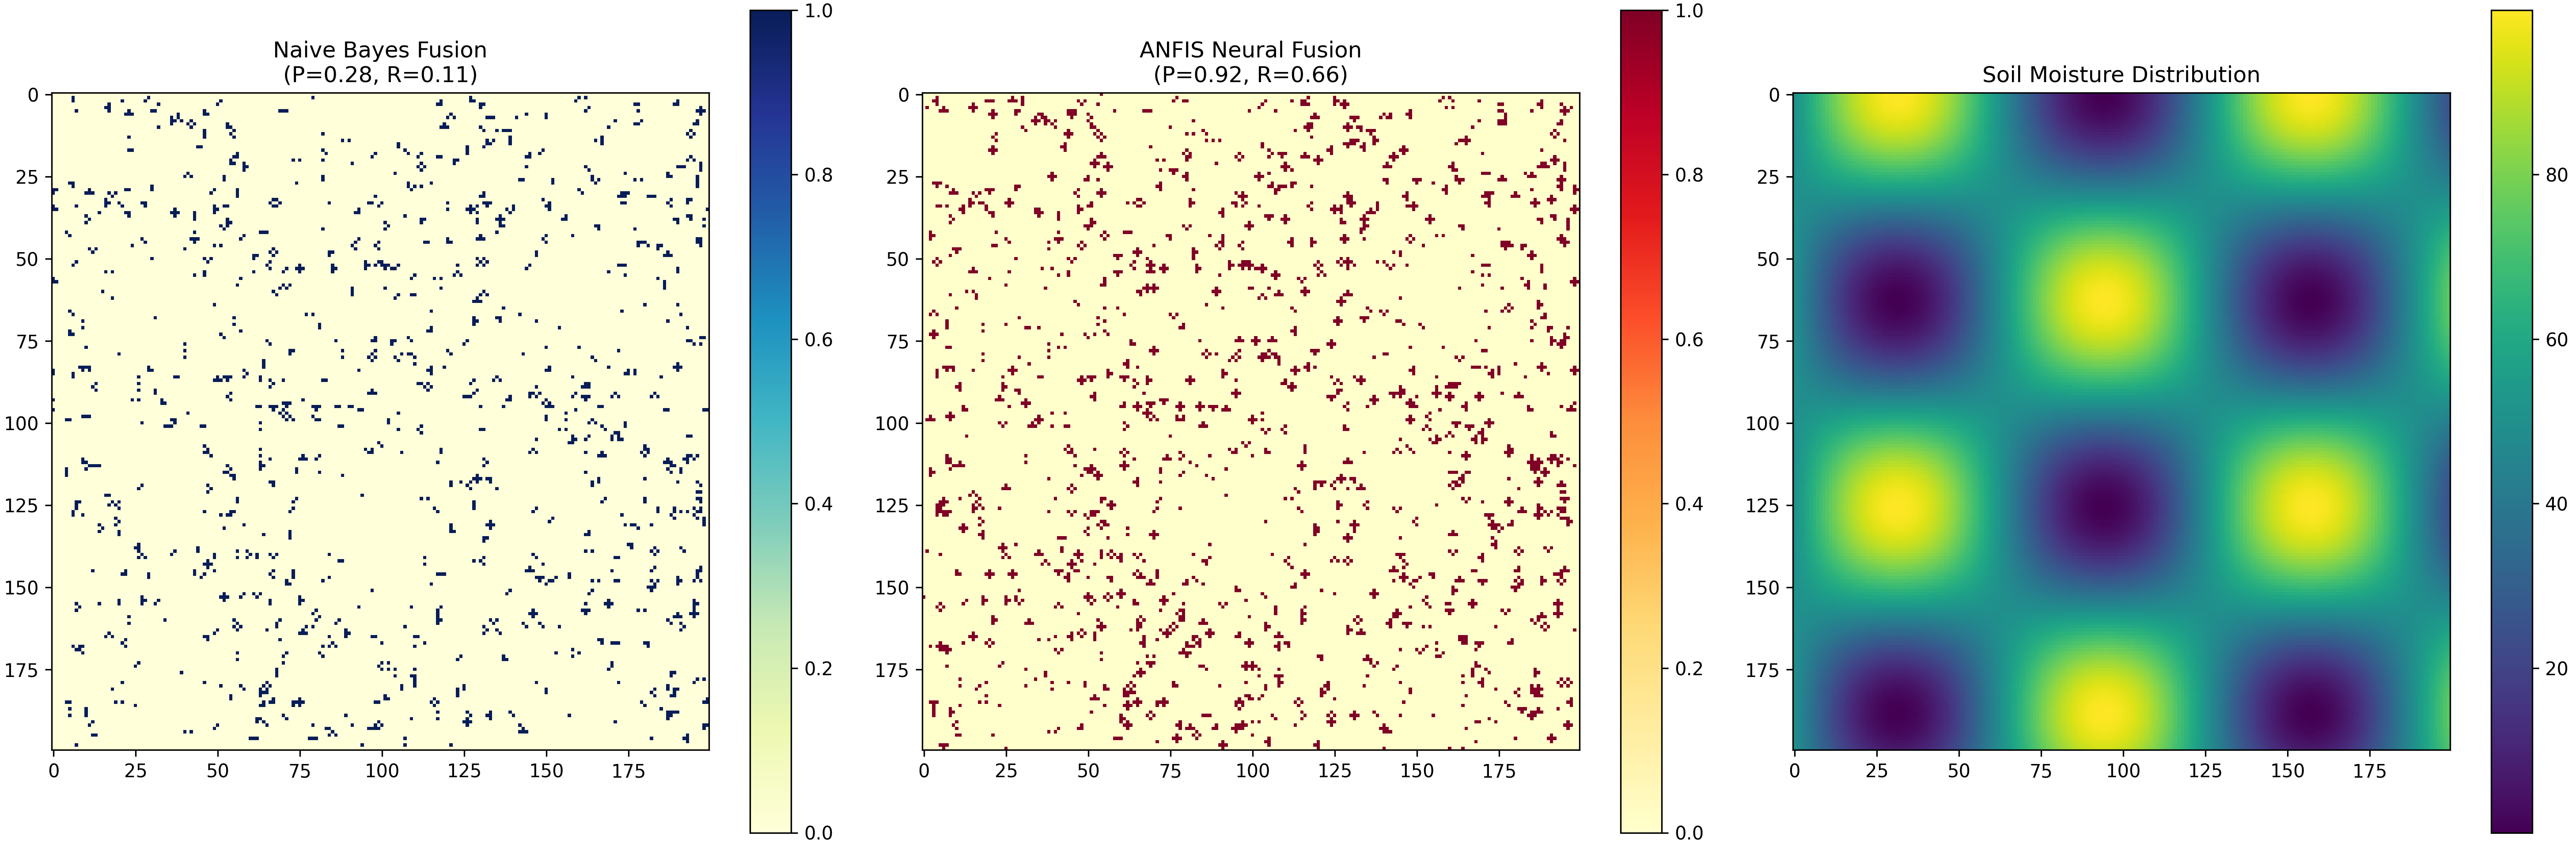
\includegraphics[width=0.98\textwidth]{figs/Rory/0_summary.png}
        \caption{ANFIS NB comparison summary. \textbf{Left:} simulated fusion for Naive Bayes. \textbf{Centre:} simulated fusion for ANFIS. \textbf{Right:} soil moisture distribution}
        \label{fig:anfis_summary}
    \end{figure}

    \paragraph{Future Work} 

        Several other physics-driven fusion algorithms exist. Another such approach is \textit{Physics Based Deep Learning} (PBDL)\footnote{\url{https://www.physicsbaseddeeplearning.org/intro.html}}, which benefits from implementing the physical domain knowledge at a deeper level in the \textit{model architecture and loss function}. PBDL is a recent field in Artificial Intelligence (AI), and it may have significant benefits, such as greater robustness to environmental variations in data-fusion for the detection of landmines.




%\newpage
\fancyhead[C]{Samuel Grace}
\section{Simulation and Control} \label{simulationandcontrol}

Samuel Grace 123 \cite{cabreira2019cpp}

\newpage
\fancyhead[C]{Thomas Turner}
\section{Intra-UAV Communication Architecture} \label{Intra Communication}

\subsection{Introduction and Philosophy}
The communication and networking of devices on our device is a key consideration for design. This is because of the specific design challenges of achieving redundancy and modularity at low power and low cost. In line with these key design guidelines all interfaces and software should be as uniform as possible to reduce the training required for operation and to reduce the difficulty of creating new components for specific environments and regulations.


\subsection{Design Considerations}\label{sub_sub_section:tgt_intra_comms_design_considerations}

\subsubsection{Modularity}\label{sub_sub_section:tgt_modularity}
\paragraph{Relevance}
Mechanical modularity is the most obvious path as the components need to physically connect easily. However, the communication architecture also needs to support this so that devices can easily communicate even if they are changed completely.
\paragraph{Modular Communication Protocols}
Defined interfaces, protocols and pin allow for different devices to communicate without specific dependencies on each other. Therefore, integrating new sensors or modules does not require a new communication system. Another key property of modular networks is physical, some networks lend themselves better to modular design, for example for a \gls{CAN} FD Bus you only need to add a stub and all interfaces should use standard connectors.

\subsubsection{Telemetry}\label{sub_sub_section:tgt_telemetry}
\paragraph{Battery Telemetry}
The two key failure modes for the battery are state of charge and thermal runaway. Both can cause complete failure and therefore both should be monitored during flight. This allows for \gls{RTH} to be triggered in case of a state of charge or emergency landing in the case of thermal runaway. Therefore, real-time telemetry is sent from the \gls{BMS} to the flight controller for temperature and state of charge.
\paragraph{\gls{ESC} Telemetry}
Providing \gls{ESC} telemetry for voltage, current and \gls{RPM} is important information when classifying motor and propeller faults accurately which is needed to support the adaptive control strategy in Section \ref{sub_sub_section:tgt_actuator_fault}. Furthermore, \gls{ESC} temperature is also sent to monitor for overheating. 

\subsubsection{Communication Bus}\label{sub_sub_section:tgt_bus}
\paragraph{\gls{CAN} bus}
In order to support the \gls{ESC} telemetry required Cyphal should be used as it is widely supported by \gls{COTS} hardware and can run over \gls{CAN} bus. CAN Flexible Data (FD) is widely used and supported and can process data transfer speeds up to 8 Mbps using the transceiver used in Section \ref{section:Custom Hardware}\footnote{\url{https://www.ti.com/lit/ds/symlink/tcan1472-q1.pdf}} whilst also supporting modularity. In order to guarantee redundancy a dual \gls{CAN} bus is selected so if there is a failure on one bus, the other bus is used. Failures can be detected across the bus as all modules will communicate 10 Hz heartbeats to each other indicating that they are operating as normal so if this heartbeat is not received the redundant bus is used instead. This allows for failure handovers in just 0.1s. Lastly, as \gls{CAN} is a differential signal the lines are carried in a twisted pair and transferred in a sheaf to reduce \gls{EMI} and risk of damage. 
\paragraph{Imaging Separation}
The images used in GPR and Thermal require significantly more data then both telemetry and command signals. Therefore, they are separately connected to the on-board computer using 1000BASE-T Gigabit Ethernet supporting data transfer speeds up to 1 Gbps. It also utilises a copper twisted pair and differential signal for noise rejection \cite{Ethernet}.  This supports thermal and GPR imaging in addition to future upgrades and increased data transfer rates.
\paragraph{Node Distribution}
Safety critical devices ensure that the drone does not sustain damage or isolate itself. This includes components necessary for flight and the sensors required for \gls{RTS} explored in Section \ref{Return to Safety}. To ensure that failures are minimised, safety critical devices should be redundant. If a safety critical device does not have a redundant version it should be able to communicate on at least two different lines preventing a single module failure causing device failure. Distributing the devices on different communication lines reduces the risk of failure as it reduces the risk of common mode failure. For example, if a \gls{GNSS} module were to have an improper fixture and move in a way that it severs all connections; if both communication lines are in it, both are severed. However, if it is on only one communication line then the other communication line is undamaged. This layout is shown in Figure \ref{fig:CAN_bus}. 
 \begin{figure}[h]
 \centering
  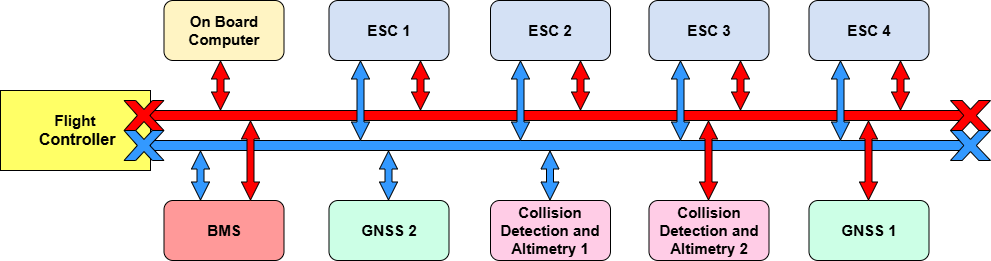
\includegraphics[width=1\textwidth]{figs/Thomas/Intra Communication/CAN bus.png}
 \caption{Bus layout}
 \label{fig:CAN_bus}
 \end{figure}
\paragraph{Communication Architecture}
Centralised architectures consist of a central node directly connected to all the relevant devices. while this is a simple and cost effective method it leaves the device to single points of failure. In order to build robustness, the custom \gls{GNSS} module is capable of independently executing landing and \gls{RTS} as it is equipped with an independent \gls{IMU} that is control capable. The \gls{GNSS} module sends control signals if the flight controller is no longer received ensuring smooth handover. 
\paragraph{High Level Protocol}
A single high level protocol being used across all components makes the \gls{UAV} more adaptable and makes hiring developers easier. This is because a single skill-set can interact with the entire system. Therefore, Cyphal will be used as it can operate over \gls{CAN} and Ethernet which are the key communication systems. It is used over alternative application protocols including ROS 2 and Mavlink as it has wider support from \gls{COTS} \gls{ESC}s\footnote{\url{https://opencyphal.org/}} . 
\subsection{Protocol Selection}\label{sub_section:tgt_protocol_selection}

\subsubsection{Requirements and Options}\label{sub_sub_section:tgt_requirements}
\paragraph{Message Requirements}
Table \ref{tab:messages} shows the required messages for flight and imaging. From this it is clear that imaging requires a far higher data transfer speeds. This means a network of low speed modules could be used with a separate imaging network.
\begin{table}[h]
\centering
\begin{tabular}{|c|c|c|c|c|c|c|} 
\hline
\textbf{Protocol} & \textbf{Speed} & \textbf{Complexity} & \textbf{Power Draw} & \textbf{Noise Tolerance} & \textbf{Cost} & \textbf{Use Case} \\ 
\hline 
CAN FD & 5 Mbps & Medium & Medium & High & Medium & Bus \\ 
FlexRay & 10 Mbps & High & High & High & High & Bus \\ 
I$^2$C & 400 Kbps & Low & Low & Low & Low & Sensors \\ 
SPI & 100 Mbps & Medium & Low & Medium & Low & Sensors \\ 
UART & 1 Mbps & Low & Low & Low & Low & Sensors \\ 
Ethernet & 1 Gbps & Medium & Medium & High & Medium & Imaging \\ 
\hline 
\end{tabular}
\caption{Communication Protocols}
\label{tab:communication_options}
\end{table}
\begin{table}[h]
\centering
\begin{tabular}{|c|c|c|c|c|} 
\hline
\textbf{Purpose}&\textbf{Frequency (Hz)}&\textbf{Message Size(bits)}&\textbf{Quantity}&\textbf{Bandwidth (kbps)}\\
\hline
ESC Duty Cycle&400&16&4&25.6\\
ESC Telemetry&10&64&4&2.56\\
Fault ESC Telemetry&400&64&4&102.4\\
Imaging Location&100&48&1&4.8\\
BMS Telemetry&10&32&1&0.32\\
GNSS location&10&48&2&0.96\\
Collision Detection&100&16&2&3.2\\
GNSS Correction&1&500&1&0.5\\
\hline
\end{tabular}
\caption{Required Standard Messages}
\label{tab:device_comms_requirementsl}
\end{table}



\subsubsection{Communication between Modules}\label{sub_sub_section:tgt_comms_modules}
\paragraph{Architecture}
Centralised architectures consist of a central node directly connected to all the relevant devices, creating a single point of failure. while this is a simple and cost effective method it leaves the device to single points of failure. In order to build robustness, the custom \gls{GNSS} module is capable of independently executing landing and \gls{RTS}.  
\paragraph{Bus Selection}
FlexRay has some clear advantages including built in redundancy and higher data transfer speeds as shown in Table \ref{tab:communication_options}. However, due to its added complexity, cost and the fact it is compatible with far fewer components, a \gls{CAN} bus is the better option. This may change if the data transfer rates needed to increase or if the technology behind FlexRay becomes cheaper and more widespread. Further, there are two key options for \gls{CAN}, time triggered or flexible data. Time triggered is an attractive as it supports higher data transfer rates however, flexible data is more widely supported and is sufficient for the application.\cite{CANFlexRay}
 
\subsubsection{Communication with sensors}\label{sub_sub_section:tgt_comms_sensors}
\paragraph{High Speed Sensors}
The simple but high speed \gls{SPI} protocol should be used whenever possible. This is because it is widely supporting by commercially available sensors and \gls{MCU}s. Uniformly using similar sensor sets also has the benefit of simplicity of implementation.
\paragraph{Low Speed Sensors}
Both \gls{UART} and \gls{I$^2$C} are widely supported, both are simple and effective however, \gls{UART} is slightly wider supported therefore on non-complex modules is used where possible. However, if pins are limited \gls{I$^2$C} should be used as it can bus multiple low speed sensors.
\paragraph{Memory Devices}
MicroSD and SD cards can communicate with \gls{SPI} or \gls{SDIO}. \gls{SPI} uses 1 bit writing and \gls{SDIO} uses 4 bit communication making \gls{SDIO} faster but harder to design traces with\footnote{\url{https://fmuser.org/news/IPTV-encoder/Introduction-to-SPI-I2C-UART-I2S-GPIO-SDIO-CAN/}}. Therefore, for the flight controller \gls{SPI} was used as the data transfer rates are low. However, while recording imaging data on the main computers SD card, \gls{SDIO} should be used in order to support the high writing speeds required. 
\paragraph{Imaging Sensors}
The imaging sensors require very high data transfer rates of over 34 mbps and are not safety critical. They are therefore not included on the \gls{CAN} bus but instead directly connect to the onboard computer using Ethernet as it can handle the higher speeds required.
\paragraph{Debugger}
Debugging is possible using the \gls{CAN} bus at a system level but for in depth on board debugging that might be required for failure analysis or uploading code to boards should also be available.\gls{UART} can be used as a live signal monitor similar to CAN however, for full access debugging a \gls{SWD} interface is used\footnote{\url{https://runtimerec.com/using-debugging-interfaces-uart-jtag-and-swd-demystified}}. Therefore, for system wide debugging the \gls{CAN} bus will be used, and for onboard debugging a \gls{SWD} will be used.
\paragraph{High Level Protocol}
A single high level protocol being used across all components makes the \gls{UAV} more adaptable and makes hiring developers easier. This is because a single skill-set can interact with the entire system. Therefore, Cyphal will be used as it can operate over \gls{CAN} and Ethernet \footnote{\url{https://opencyphal.org/}} which are the key communication systems. 


%\newpage
\fancyhead[C]{Rory Millard}
\section{Project Financing} \label{financing}

% --- Introduction: Clearer statement of purpose ---
This section presents an economic analysis comparing the drone-based landmine detection system proposed in this report with legacy manual metal-detector methods, focusing on the cost-effectiveness for surveying \textbf{and demining} operations near Kharkiv, Ukraine. The metric for comparison is the total cost to survey and clear one square kilometre (km²) of land, to a recall of over 90\%. The analysis links the system's financial improvement over the legacy system with sensor performance metrics $P_{sys}$ and $R_{sys}$.


\subsection{Cost Comparison} \label{subsec:cost_structures}

The capital costs of the drone-based system proposed in this report are higher than that of legacy manual techniques, which don't rely on expensive equipment, except from transportation and metal detectors. However, for each system, the operational costs are significantly higher than the upfront capital costs due to the labour intensive surveying and clearance stages. Therefore, to compare the two systems financially, only the operational costs need to be compared, as the capital costs are small in comparison. Operational costs especially dominate if the system is leased out instead of purchased.

Legacy demining operations involve a technical survey phase costing $C_\text{legacy survey} = \$305,000 \text{ per km}^2$ surveyed, followed by a clearance phase with a nominal cost of $C_\text{clearance} = \$2,940,000 \text{ per km}^2$ cleared, according to a report from the Kyiv School of Economics\footnote{\url{https://kse.ua/wp-content/uploads/2023/09/Mining-brief_Final-1.pdf}}. Manual technical surveys typically result in clearing approximately 50\% of the surveyed area, representing a precision improvement of 2$\times$ over indiscriminate 'blind' clearance. This is significantly lower than the 27.7$\times$ estimated for the proposed system in Section \ref{fusion_bounds}. The operational cost of technical survey and clearance for legacy manual methods is estimated as:
\begin{equation}
C_{\text{legacy}} = C_{\text{legacy survey}} + (0.5 \times C_{\text{clearance}}) = \$305,000 + (0.5 \times \$2,940,000) = \$1,775,000 \text{/km}^2 
\end{equation}
The operational cost associated with surveying using the proposed drone-based system needs to be estimated. Operation involves one person working 7 hours per day, which is the high thermal contrast window detailed in Section \ref{compvis_thermalsims}. The thermal drone's scanning rate is 62 m$^2$ every 5 seconds (Section \ref{thermal_selection}). Assuming radar scans can be performed approximately concurrently, the survey duration for 1 km$^2$ is estimated at $\approx$ 4 days. With an operator wage of \$15/hr, the labour cost amounts to approximately \$500/km$^2$. The cost of electricity for battery charging is considered negligible in comparison. The expected system wear and tear must also be factored in, as it represents a large operational cost. This is difficult to quantify precisely without field trials, but the cost is estimated at \$1000/km$^2$. Consequently, the total estimated operational survey cost for the drone-based system is approximately \$1500/km$^2$.

To compare the drone system with legacy methods, the cost of clearing a flagged region is assumed to depend only on the region's area. The total operational cost for the drone system $C_{\text{drone}}$, is therefore determined by the number of flagged points, which is a function of $P_\text{sys}$ and $R_\text{sys}$, as described in Section \ref{subsec:performance_savings}. Table \ref{tab:cost_comparison_structured} presents a comparison of the estimated \textbf{operational} costs.

\begin{table}[h!]
% Removed \small command
\centering
\caption[Operational Cost Comparison]{Operational Cost Comparison: Single Drone-Based System vs. Single Manual Deminer in Kharkiv, Ukraine}
\label{tab:cost_comparison_structured}
\begin{tabular}{lcc} 
\toprule
\textbf{Cost Description} & \textbf{Drone System} & \textbf{Legacy System} \\
\midrule
\multicolumn{3}{l}{}\\
Technical Survey Cost (/km²) & \$1500 & \$305,000 \\ 
Time for Technical Survey (days/km²) &  4 & 2500 \tablefootnote{\url{https://apopo.org/what-we-do/detecting-landmines-and-explosives/how-we-do-it/mine-clearance/}} \\ 
Fraction Flagged for Clearance & 3.6\% & 50\% \\ 
Cost of Clearance (/km²) & \$106,137 & \$1,470,000 \\
 \addlinespace
\textbf{Total Cost to Demine 1 km² } & \textbf{\$107,637} & \textbf{\$1,775,000}  \\
\bottomrule
\end{tabular}
\end{table}

\subsection{Financials of System Performance} \label{subsec:performance_savings}

The operational cost of the proposed system depends on the number of point flagged for mine clearance. This depends on the initial mine density $\rho_0$, and the system's precision $P_{sys}$ and recall $R_{sys}$. The fraction of land flagged for mine clearance ($A_\text{flagged}$) is:
\begin{equation}
A_{\text{flagged}} = \frac{\text{Area Flagged}}{\text{Total Area}} \approx  \frac{\rho_0 R_\text{sys}}{P_\text{sys}}. 
\label{eq:flags_fraction} % Renamed label for clarity
\end{equation}
Given the assumption that the clearance cost just depends on the size of the flagged area, the total operational cost for the drone system per km² ($C_{\text{drone}}$) is:
\begin{equation}
C_{\text{drone}}(P_\text{sys}, R_\text{sys}) = C_{\text{survey}} + A_{\text{flagged}} \times C_{\text{clearance}} 
\approx \$1480 + \left( \frac{\rho_0 R_\text{sys}}{P_\text{sys}} \right) \times \$2,940,000 
\label{eq:drone_op_cost} % New label
\end{equation}



Equation \ref{eq:drone_op_cost} demonstrates that improving $P_{sys}$ results in a large operational cost reduction by reducing the number of points flagged for mine removal. While maximizing recall $R_{sys}$ is important for safety (as discussed in Section \ref{lossmatrix}), achieving high precision is the only way the system can be economically viable. The cost savings by choosing the proposed system over legacy systems are plotted in Figure \ref{fig:financial_savings} as a function of $P_\text{sys}$ and $R_\text{sys}$. The expected region of system performance is also plotted (using the bounds from Section \ref{fusion_bounds}), indicating an \textbf{expected operational cost saving of between $\approx$ \$1.65~m - \$1.75~m per km²} surveyed, over the legacy operational cost of \$1.775~m/km². 


% --- Figure - Needs updated caption reflecting source of data/need for recalc ---
\begin{figure}[h!]
\centering
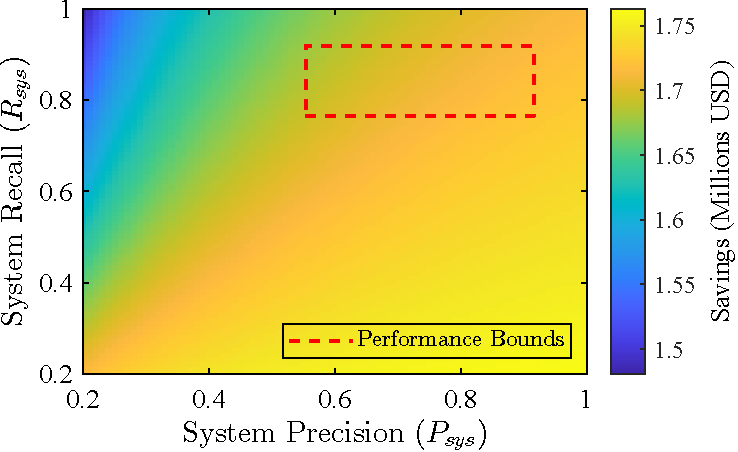
\includegraphics[width=0.5\textwidth]{figs/Rory/financial_savings.pdf} 
\caption[Operational Cost Savings as a Function of Computer Vision Performance]{Plot of Equation \ref{eq:drone_op_cost}. Operational cost savings of the proposed system over legacy systems for surveying and demining 1~km$^2$, varying with $P_{sys}$ and $R_{sys}$. The expected system performance from Section \ref{fusion_bounds} is the region inside the dashed rectangle.}
\label{fig:financial_savings}
\end{figure}


\subsection{Conclusion} \label{subsec:finance_conclusion}

This section strongly suggests that the drone-based detection system proposed in this report offers significant financial benefits over legacy manual demining techniques. The operational costs are reduced by a factor of over 20$\times$, whilst the system is significantly faster. The improved precision means that the area flagged for clearance is much smaller than in legacy techniques, which causes a large reduction in the most significant part of the operational costs and times. These reductions in cost and time will enable more widespread demining operations, restoring large areas of productive land, and saving countless lives. 

Future work should investigate more accurate cost estimates. For the operational costs, more advanced YOLOv11 models (Section \ref{compvis_implementation}) should be trained on real world experimental data. The ANFIS network (Section \ref{fusion}) should be implemented, and the performance metrics $P_\text{sys}$ and $R_\text{sys}$ should be found by testing the entire system on a large dataset of unseen experimental data. This would give a more accurate picture of the system's financial viability, which would help in securing funding if the project were commercialised.



\fancyhead[C]{Student}
\printbibliography{biblio}

% Appendix
% Essential content that interrupts the flow of the document can be placed here, e.g. technical drawings, detailed lists of equations used, etc.
\newpage
\addcontentsline{toc}{section}{Appendix}
\section*{Appendix}

\end{document}
